% Options for packages loaded elsewhere
\PassOptionsToPackage{unicode}{hyperref}
\PassOptionsToPackage{hyphens}{url}
\PassOptionsToPackage{dvipsnames,svgnames*,x11names*}{xcolor}
%
\documentclass[
]{article}
\usepackage{lmodern}
\usepackage{amssymb,amsmath}
\usepackage{ifxetex,ifluatex}
\ifnum 0\ifxetex 1\fi\ifluatex 1\fi=0 % if pdftex
  \usepackage[T1]{fontenc}
  \usepackage[utf8]{inputenc}
  \usepackage{textcomp} % provide euro and other symbols
\else % if luatex or xetex
  \usepackage{unicode-math}
  \defaultfontfeatures{Scale=MatchLowercase}
  \defaultfontfeatures[\rmfamily]{Ligatures=TeX,Scale=1}
\fi
% Use upquote if available, for straight quotes in verbatim environments
\IfFileExists{upquote.sty}{\usepackage{upquote}}{}
\IfFileExists{microtype.sty}{% use microtype if available
  \usepackage[]{microtype}
  \UseMicrotypeSet[protrusion]{basicmath} % disable protrusion for tt fonts
}{}
\makeatletter
\@ifundefined{KOMAClassName}{% if non-KOMA class
  \IfFileExists{parskip.sty}{%
    \usepackage{parskip}
  }{% else
    \setlength{\parindent}{0pt}
    \setlength{\parskip}{6pt plus 2pt minus 1pt}}
}{% if KOMA class
  \KOMAoptions{parskip=half}}
\makeatother
\usepackage{xcolor}
\IfFileExists{xurl.sty}{\usepackage{xurl}}{} % add URL line breaks if available
\IfFileExists{bookmark.sty}{\usepackage{bookmark}}{\usepackage{hyperref}}
\hypersetup{
  pdftitle={Skills Problem Set 1},
  pdfauthor={Fernanda Sobrino},
  colorlinks=true,
  linkcolor=Maroon,
  filecolor=Maroon,
  citecolor=Blue,
  urlcolor=blue,
  pdfcreator={LaTeX via pandoc}}
\urlstyle{same} % disable monospaced font for URLs
\usepackage[margin=1in]{geometry}
\usepackage{color}
\usepackage{fancyvrb}
\newcommand{\VerbBar}{|}
\newcommand{\VERB}{\Verb[commandchars=\\\{\}]}
\DefineVerbatimEnvironment{Highlighting}{Verbatim}{commandchars=\\\{\}}
% Add ',fontsize=\small' for more characters per line
\usepackage{framed}
\definecolor{shadecolor}{RGB}{248,248,248}
\newenvironment{Shaded}{\begin{snugshade}}{\end{snugshade}}
\newcommand{\AlertTok}[1]{\textcolor[rgb]{0.94,0.16,0.16}{#1}}
\newcommand{\AnnotationTok}[1]{\textcolor[rgb]{0.56,0.35,0.01}{\textbf{\textit{#1}}}}
\newcommand{\AttributeTok}[1]{\textcolor[rgb]{0.77,0.63,0.00}{#1}}
\newcommand{\BaseNTok}[1]{\textcolor[rgb]{0.00,0.00,0.81}{#1}}
\newcommand{\BuiltInTok}[1]{#1}
\newcommand{\CharTok}[1]{\textcolor[rgb]{0.31,0.60,0.02}{#1}}
\newcommand{\CommentTok}[1]{\textcolor[rgb]{0.56,0.35,0.01}{\textit{#1}}}
\newcommand{\CommentVarTok}[1]{\textcolor[rgb]{0.56,0.35,0.01}{\textbf{\textit{#1}}}}
\newcommand{\ConstantTok}[1]{\textcolor[rgb]{0.00,0.00,0.00}{#1}}
\newcommand{\ControlFlowTok}[1]{\textcolor[rgb]{0.13,0.29,0.53}{\textbf{#1}}}
\newcommand{\DataTypeTok}[1]{\textcolor[rgb]{0.13,0.29,0.53}{#1}}
\newcommand{\DecValTok}[1]{\textcolor[rgb]{0.00,0.00,0.81}{#1}}
\newcommand{\DocumentationTok}[1]{\textcolor[rgb]{0.56,0.35,0.01}{\textbf{\textit{#1}}}}
\newcommand{\ErrorTok}[1]{\textcolor[rgb]{0.64,0.00,0.00}{\textbf{#1}}}
\newcommand{\ExtensionTok}[1]{#1}
\newcommand{\FloatTok}[1]{\textcolor[rgb]{0.00,0.00,0.81}{#1}}
\newcommand{\FunctionTok}[1]{\textcolor[rgb]{0.00,0.00,0.00}{#1}}
\newcommand{\ImportTok}[1]{#1}
\newcommand{\InformationTok}[1]{\textcolor[rgb]{0.56,0.35,0.01}{\textbf{\textit{#1}}}}
\newcommand{\KeywordTok}[1]{\textcolor[rgb]{0.13,0.29,0.53}{\textbf{#1}}}
\newcommand{\NormalTok}[1]{#1}
\newcommand{\OperatorTok}[1]{\textcolor[rgb]{0.81,0.36,0.00}{\textbf{#1}}}
\newcommand{\OtherTok}[1]{\textcolor[rgb]{0.56,0.35,0.01}{#1}}
\newcommand{\PreprocessorTok}[1]{\textcolor[rgb]{0.56,0.35,0.01}{\textit{#1}}}
\newcommand{\RegionMarkerTok}[1]{#1}
\newcommand{\SpecialCharTok}[1]{\textcolor[rgb]{0.00,0.00,0.00}{#1}}
\newcommand{\SpecialStringTok}[1]{\textcolor[rgb]{0.31,0.60,0.02}{#1}}
\newcommand{\StringTok}[1]{\textcolor[rgb]{0.31,0.60,0.02}{#1}}
\newcommand{\VariableTok}[1]{\textcolor[rgb]{0.00,0.00,0.00}{#1}}
\newcommand{\VerbatimStringTok}[1]{\textcolor[rgb]{0.31,0.60,0.02}{#1}}
\newcommand{\WarningTok}[1]{\textcolor[rgb]{0.56,0.35,0.01}{\textbf{\textit{#1}}}}
\usepackage{graphicx,grffile}
\makeatletter
\def\maxwidth{\ifdim\Gin@nat@width>\linewidth\linewidth\else\Gin@nat@width\fi}
\def\maxheight{\ifdim\Gin@nat@height>\textheight\textheight\else\Gin@nat@height\fi}
\makeatother
% Scale images if necessary, so that they will not overflow the page
% margins by default, and it is still possible to overwrite the defaults
% using explicit options in \includegraphics[width, height, ...]{}
\setkeys{Gin}{width=\maxwidth,height=\maxheight,keepaspectratio}
% Set default figure placement to htbp
\makeatletter
\def\fps@figure{htbp}
\makeatother
\setlength{\emergencystretch}{3em} % prevent overfull lines
\providecommand{\tightlist}{%
  \setlength{\itemsep}{0pt}\setlength{\parskip}{0pt}}
\setcounter{secnumdepth}{5}

\title{Skills Problem Set 1}
\author{Fernanda Sobrino}
\date{3/14/2021}

\begin{document}
\maketitle

Due Thursday April 8, midnight Central Time.

Upload your pdf to canvas.

Push your code to your repo on Github Classroom.

This submission is my work alone and complies with the 30535 integrity
policy.

Add your initials to indicate your agreement: \textbf{ES}

Add names of anyone you discussed this problem set with:

\textbf{Guillermo Antonio Trefogli Wong}

Late coins used this pset: 0. Late coins left after submission: 9.

Name your submission files \texttt{skills\_ps\_1.Rmd} and
\texttt{skills\_ps\_1.pdf}. (10 points)

\hypertarget{setup}{%
\section{Setup}\label{setup}}

\hypertarget{installation-10-points}{%
\subsection{Installation (10 points)}\label{installation-10-points}}

\begin{enumerate}
\def\labelenumi{\arabic{enumi}.}
\tightlist
\item
  If you do not have R and RStudio installed:watch and follow the video
  on how to install them
\item
  If you do not have a github account, set up one now
\item
  Download Github Desktop \href{https://desktop.github.com/}{here}. If
  you are familiar with using \texttt{git} through the command line you
  are welcome to do so.
\item
  Initialize your ps1 repository and download the pset\_template
  \href{https://classroom.github.com/a/HL4qfScl}{here}. Please read the
  README file which is visible on the repo's homepage.
\item
  Make sure you already installed these packages in R:
  \texttt{tidyverse}, \texttt{markdown}, and \texttt{dslabs}
\end{enumerate}

\begin{Shaded}
\begin{Highlighting}[]
\CommentTok{# install.packages("tidyverse")}
\CommentTok{# install.packages("markdown")}
\CommentTok{# install.packages("dslabs")}

\CommentTok{## First specify the packages of interest}
\NormalTok{list.of.packages <-}\StringTok{ }\KeywordTok{c}\NormalTok{(}\StringTok{"tidyverse"}\NormalTok{, }\StringTok{"markdown"}\NormalTok{, }\StringTok{"dslabs"}\NormalTok{)}

\CommentTok{## Now load or install&load all}
\NormalTok{package.check <-}\StringTok{ }\KeywordTok{lapply}\NormalTok{(}
\NormalTok{  list.of.packages,}
  \DataTypeTok{FUN =} \ControlFlowTok{function}\NormalTok{(x) \{}
    \ControlFlowTok{if}\NormalTok{ (}\OperatorTok{!}\KeywordTok{require}\NormalTok{(x, }\DataTypeTok{character.only =} \OtherTok{TRUE}\NormalTok{)) \{}
      \KeywordTok{install.packages}\NormalTok{(x, }\DataTypeTok{dependencies =} \OtherTok{TRUE}\NormalTok{)}
      \KeywordTok{library}\NormalTok{(x, }\DataTypeTok{character.only =} \OtherTok{TRUE}\NormalTok{)}
\NormalTok{    \}}
\NormalTok{  \}}
\NormalTok{)}
\end{Highlighting}
\end{Shaded}

\begin{verbatim}
## Loading required package: markdown
\end{verbatim}

\begin{verbatim}
## Warning: package 'markdown' was built under R version 4.0.5
\end{verbatim}

\begin{enumerate}
\def\labelenumi{\arabic{enumi}.}
\tightlist
\item
  Run a line of code which tests the packages are installed using
  Stackoverflow instructions posted
  \href{https://stackoverflow.com/questions/4090169/elegant-way-to-check-for-missing-packages-and-install-them}{here}.
\end{enumerate}

\begin{Shaded}
\begin{Highlighting}[]
\NormalTok{list.of.packages <-}\StringTok{ }\KeywordTok{c}\NormalTok{(}\StringTok{"tidyverse"}\NormalTok{, }\StringTok{"markdown"}\NormalTok{, }\StringTok{"dslabs"}\NormalTok{)}
\NormalTok{new.packages <-}\StringTok{ }\NormalTok{list.of.packages[}\OperatorTok{!}\NormalTok{(list.of.packages }\OperatorTok\StringTok{ }\KeywordTok{installed.packages}\NormalTok{()[,}\StringTok{"Package"}\NormalTok{])]}
\ControlFlowTok{if}\NormalTok{(}\KeywordTok{length}\NormalTok{(new.packages)) }\KeywordTok{install.packages}\NormalTok{(new.packages)}
\end{Highlighting}
\end{Shaded}

Put the output in your problem set. This lets us know which packages
successfully installed and which ones didn't 1. What is your github id?

My github id is guccimane457

\begin{enumerate}
\def\labelenumi{\arabic{enumi}.}
\tightlist
\item
  Add and commit your code. Push it to github with commit message
  ``start-up completed''
\end{enumerate}

Please check Github for my commits.

\begin{enumerate}
\def\labelenumi{\arabic{enumi}.}
\tightlist
\item
  Now we'll practice reverting.

  \begin{enumerate}
  \def\labelenumii{\alph{enumii}.}
  \tightlist
  \item
    Add the following text to you homework: ``Why did the code on Github
    delete tindr?''
  \item
    Now push the code to Github.
  \item
    Now revert to the previous state of the code. (Now that the code is
    uncommitted, maybe it'll join tindr again.)
  \end{enumerate}
\end{enumerate}

Please check Github for my commits.

\hypertarget{r-for-data-science-exercises}{%
\section{R for Data Science
Exercises}\label{r-for-data-science-exercises}}

\hypertarget{first-steps-10-points}{%
\subsection{First Steps (10 points)}\label{first-steps-10-points}}

Load \texttt{tidyverse} and \texttt{dslabs}

\begin{Shaded}
\begin{Highlighting}[]
\KeywordTok{library}\NormalTok{(tidyverse)}
\KeywordTok{library}\NormalTok{(dslabs)}
\end{Highlighting}
\end{Shaded}

We will be using \texttt{polls\_us\_election\_2016} data that is in the
\texttt{dslabs} package

\begin{enumerate}
\def\labelenumi{\arabic{enumi}.}
\tightlist
\item
  How many rows are there in \texttt{polls\_us\_election\_2016}? How
  many columns? What do the rows represent? How about the columns
\end{enumerate}

\begin{Shaded}
\begin{Highlighting}[]
\KeywordTok{glimpse}\NormalTok{(polls_us_election_}\DecValTok{2016}\NormalTok{)}
\end{Highlighting}
\end{Shaded}

\begin{verbatim}
## Rows: 4,208
## Columns: 15
## $ state            <fct> U.S., U.S., U.S., U.S., U.S., U.S., U.S., U.S., Ne...
## $ startdate        <date> 2016-11-03, 2016-11-01, 2016-11-02, 2016-11-04, 2...
## $ enddate          <date> 2016-11-06, 2016-11-07, 2016-11-06, 2016-11-07, 2...
## $ pollster         <fct> ABC News/Washington Post, Google Consumer Surveys,...
## $ grade            <fct> A+, B, A-, B, B-, A, A-, A-, NA, A-, A+, A-, A+, B...
## $ samplesize       <int> 2220, 26574, 2195, 3677, 16639, 1295, 1426, 1282, ...
## $ population       <chr> "lv", "lv", "lv", "lv", "rv", "lv", "lv", "lv", "l...
## $ rawpoll_clinton  <dbl> 47.00, 38.03, 42.00, 45.00, 47.00, 48.00, 45.00, 4...
## $ rawpoll_trump    <dbl> 43.00, 35.69, 39.00, 41.00, 43.00, 44.00, 41.00, 4...
## $ rawpoll_johnson  <dbl> 4.00, 5.46, 6.00, 5.00, 3.00, 3.00, 5.00, 6.00, 6....
## $ rawpoll_mcmullin <dbl> NA, NA, NA, NA, NA, NA, NA, NA, NA, NA, NA, NA, NA...
## $ adjpoll_clinton  <dbl> 45.20163, 43.34557, 42.02638, 45.65676, 46.84089, ...
## $ adjpoll_trump    <dbl> 41.72430, 41.21439, 38.81620, 40.92004, 42.33184, ...
## $ adjpoll_johnson  <dbl> 4.626221, 5.175792, 6.844734, 6.069454, 3.726098, ...
## $ adjpoll_mcmullin <dbl> NA, NA, NA, NA, NA, NA, NA, NA, NA, NA, NA, NA, NA...
\end{verbatim}

\begin{Shaded}
\begin{Highlighting}[]
\CommentTok{# conversely, you can also use ncol() and nrow() to find out how many rows and }
\CommentTok{# columns there are.}

\KeywordTok{view}\NormalTok{(polls_us_election_}\DecValTok{2016}\NormalTok{)}

\KeywordTok{summary}\NormalTok{(polls_us_election_}\DecValTok{2016}\NormalTok{)}
\end{Highlighting}
\end{Shaded}

\begin{verbatim}
##             state        startdate             enddate          
##  U.S.          :1106   Min.   :2015-11-06   Min.   :2015-11-08  
##  Florida       : 148   1st Qu.:2016-08-10   1st Qu.:2016-08-21  
##  North Carolina: 125   Median :2016-09-23   Median :2016-09-30  
##  Pennsylvania  : 125   Mean   :2016-08-31   Mean   :2016-09-06  
##  Ohio          : 115   3rd Qu.:2016-10-20   3rd Qu.:2016-10-28  
##  New Hampshire : 112   Max.   :2016-11-06   Max.   :2016-11-07  
##  (Other)       :2477                                            
##                                      pollster        grade     
##  Ipsos                                   : 919   A-     :1085  
##  Google Consumer Surveys                 : 743   B      :1011  
##  SurveyMonkey                            : 660   C-     : 693  
##  YouGov                                  : 130   C+     : 329  
##  Rasmussen Reports/Pulse Opinion Research: 125   B+     : 204  
##  USC Dornsife/LA Times                   : 121   (Other): 457  
##  (Other)                                 :1510   NA's   : 429  
##    samplesize       population        rawpoll_clinton rawpoll_trump  
##  Min.   :   35.0   Length:4208        Min.   :11.04   Min.   : 4.00  
##  1st Qu.:  447.5   Class :character   1st Qu.:38.00   1st Qu.:35.00  
##  Median :  772.0   Mode  :character   Median :43.00   Median :40.00  
##  Mean   : 1148.2                      Mean   :41.99   Mean   :39.83  
##  3rd Qu.: 1236.5                      3rd Qu.:46.20   3rd Qu.:45.00  
##  Max.   :84292.0                      Max.   :88.00   Max.   :68.00  
##  NA's   :1                                                           
##  rawpoll_johnson  rawpoll_mcmullin adjpoll_clinton adjpoll_trump   
##  Min.   : 0.000   Min.   : 9.0     Min.   :17.06   Min.   : 4.373  
##  1st Qu.: 5.400   1st Qu.:22.5     1st Qu.:40.21   1st Qu.:38.429  
##  Median : 7.000   Median :25.0     Median :44.15   Median :42.765  
##  Mean   : 7.382   Mean   :24.0     Mean   :43.32   Mean   :42.674  
##  3rd Qu.: 9.000   3rd Qu.:27.9     3rd Qu.:46.92   3rd Qu.:46.290  
##  Max.   :25.000   Max.   :31.0     Max.   :86.77   Max.   :72.433  
##  NA's   :1409     NA's   :4178                                     
##  adjpoll_johnson  adjpoll_mcmullin
##  Min.   :-3.668   Min.   :11.03   
##  1st Qu.: 3.145   1st Qu.:23.11   
##  Median : 4.384   Median :25.14   
##  Mean   : 4.660   Mean   :24.51   
##  3rd Qu.: 5.756   3rd Qu.:27.98   
##  Max.   :20.367   Max.   :31.57   
##  NA's   :1409     NA's   :4178
\end{verbatim}

\begin{Shaded}
\begin{Highlighting}[]
\CommentTok{# there are 4208 rows in `polls_us_election_2016`}
\CommentTok{# there are 15 columns in `polls_us_election_2016`}
 
\CommentTok{# the rows or observations represent individual polls and their characteristics }
\CommentTok{# in the U.S. / U.S. States in 2016.}

\CommentTok{# the columns represent the variables included in the dataset. }
\CommentTok{# For example, grade and population.}
\end{Highlighting}
\end{Shaded}

\begin{enumerate}
\def\labelenumi{\arabic{enumi}.}
\tightlist
\item
  Make a scatter-plot of startdate vs rawpoll\_clinton
\end{enumerate}

\begin{Shaded}
\begin{Highlighting}[]
\KeywordTok{library}\NormalTok{(ggplot2)}
\KeywordTok{qplot}\NormalTok{(}\DataTypeTok{x =} \StringTok{`}\DataTypeTok{startdate}\StringTok{`}\NormalTok{, }\DataTypeTok{y =} \StringTok{`}\DataTypeTok{rawpoll_clinton}\StringTok{`}\NormalTok{, }\DataTypeTok{data =}\NormalTok{ polls_us_election_}\DecValTok{2016}\NormalTok{)}
\end{Highlighting}
\end{Shaded}

\includegraphics{skills_ps_1_files/figure-latex/unnamed-chunk-5-1.pdf}

\begin{enumerate}
\def\labelenumi{\arabic{enumi}.}
\tightlist
\item
  What does the variable grade describes? Use the help
  `?polls\_us\_election\_2016 to find out.
\end{enumerate}

\begin{Shaded}
\begin{Highlighting}[]
\NormalTok{?polls_us_election_}\DecValTok{2016}
\end{Highlighting}
\end{Shaded}

\begin{verbatim}
## starting httpd help server ... done
\end{verbatim}

\begin{Shaded}
\begin{Highlighting}[]
\CommentTok{# According to R documentation, the variable `grade` describes Grade assigned by }
\CommentTok{# fivethirtyeight to the pollster.}
\end{Highlighting}
\end{Shaded}

\begin{enumerate}
\def\labelenumi{\arabic{enumi}.}
\tightlist
\item
  What happens if you make a scatter-plot of population and grade? Why
  is the plot not useful?
\end{enumerate}

\begin{Shaded}
\begin{Highlighting}[]
\KeywordTok{library}\NormalTok{(ggplot2)}
\KeywordTok{qplot}\NormalTok{(}\DataTypeTok{x =} \StringTok{`}\DataTypeTok{population}\StringTok{`}\NormalTok{, }\DataTypeTok{y =} \StringTok{`}\DataTypeTok{grade}\StringTok{`}\NormalTok{, }\DataTypeTok{data =}\NormalTok{ polls_us_election_}\DecValTok{2016}\NormalTok{)}
\end{Highlighting}
\end{Shaded}

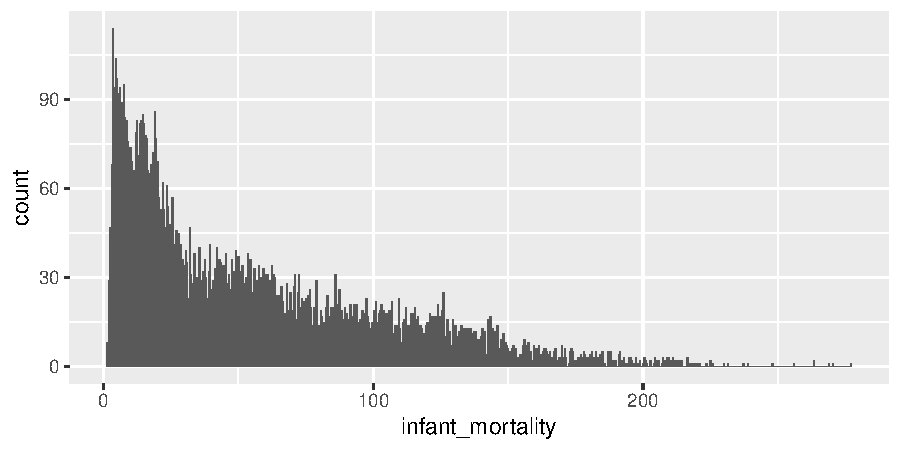
\includegraphics{skills_ps_1_files/figure-latex/unnamed-chunk-7-1.pdf}

\begin{Shaded}
\begin{Highlighting}[]
\CommentTok{# this scatter plot of population and grade is not useful because we cannot}
\CommentTok{# observe the distribution for either variable across pollsters, or some period }
\CommentTok{# range. These variables are dependent on pollsters, and they characterize }
\CommentTok{# pollsters. To observe the distribution, we must match these variables with an }
\CommentTok{# independent variable (for example, startdate and pollster)}
\end{Highlighting}
\end{Shaded}

\hypertarget{grammar-of-graphics-mapping-data-to-aesthetics-20-points}{%
\subsection{Grammar of graphics: mapping data to aesthetics (20
points)}\label{grammar-of-graphics-mapping-data-to-aesthetics-20-points}}

\begin{enumerate}
\def\labelenumi{\arabic{enumi}.}
\tightlist
\item
  Run \texttt{?polls\_us\_election\_2016} to see the documentation for
  the data set. Run \texttt{head(polls\_us\_election\_2016)} to see the
  first 6 rows of this data frame. Run
  \texttt{colnames(polls\_us\_election\_2016)} to inspect which
  variables we have for each poll
\end{enumerate}

\begin{Shaded}
\begin{Highlighting}[]
\NormalTok{?polls_us_election_}\DecValTok{2016}

\KeywordTok{head}\NormalTok{(polls_us_election_}\DecValTok{2016}\NormalTok{)}
\end{Highlighting}
\end{Shaded}

\begin{verbatim}
##   state  startdate    enddate
## 1  U.S. 2016-11-03 2016-11-06
## 2  U.S. 2016-11-01 2016-11-07
## 3  U.S. 2016-11-02 2016-11-06
## 4  U.S. 2016-11-04 2016-11-07
## 5  U.S. 2016-11-03 2016-11-06
## 6  U.S. 2016-11-03 2016-11-06
##                                                     pollster grade samplesize
## 1                                   ABC News/Washington Post    A+       2220
## 2                                    Google Consumer Surveys     B      26574
## 3                                                      Ipsos    A-       2195
## 4                                                     YouGov     B       3677
## 5                                           Gravis Marketing    B-      16639
## 6 Fox News/Anderson Robbins Research/Shaw & Company Research     A       1295
##   population rawpoll_clinton rawpoll_trump rawpoll_johnson rawpoll_mcmullin
## 1         lv           47.00         43.00            4.00               NA
## 2         lv           38.03         35.69            5.46               NA
## 3         lv           42.00         39.00            6.00               NA
## 4         lv           45.00         41.00            5.00               NA
## 5         rv           47.00         43.00            3.00               NA
## 6         lv           48.00         44.00            3.00               NA
##   adjpoll_clinton adjpoll_trump adjpoll_johnson adjpoll_mcmullin
## 1        45.20163      41.72430        4.626221               NA
## 2        43.34557      41.21439        5.175792               NA
## 3        42.02638      38.81620        6.844734               NA
## 4        45.65676      40.92004        6.069454               NA
## 5        46.84089      42.33184        3.726098               NA
## 6        49.02208      43.95631        3.057876               NA
\end{verbatim}

\begin{Shaded}
\begin{Highlighting}[]
\KeywordTok{colnames}\NormalTok{(polls_us_election_}\DecValTok{2016}\NormalTok{)}
\end{Highlighting}
\end{Shaded}

\begin{verbatim}
##  [1] "state"            "startdate"        "enddate"          "pollster"        
##  [5] "grade"            "samplesize"       "population"       "rawpoll_clinton" 
##  [9] "rawpoll_trump"    "rawpoll_johnson"  "rawpoll_mcmullin" "adjpoll_clinton" 
## [13] "adjpoll_trump"    "adjpoll_johnson"  "adjpoll_mcmullin"
\end{verbatim}

\begin{enumerate}
\def\labelenumi{\arabic{enumi}.}
\item
  Compare the following scatter-plots. Why are the two graphs different?
  Which graph is better representation of the data?
  (\textit{You do not need to graph then to answer these questions.})

\begin{Shaded}
\begin{Highlighting}[]
\CommentTok{# Graph 1}
\KeywordTok{ggplot}\NormalTok{(}\DataTypeTok{data =}\NormalTok{ polls_us_election_}\DecValTok{2016}\NormalTok{) }\OperatorTok{+}
\StringTok{  }\KeywordTok{geom_point}\NormalTok{(}\DataTypeTok{mapping =} \KeywordTok{aes}\NormalTok{(}\DataTypeTok{x =}\NormalTok{ startdate, }
                           \DataTypeTok{y =}\NormalTok{ samplesize, }
                           \DataTypeTok{color =}\NormalTok{ rawpoll_johnson)) }
\end{Highlighting}
\end{Shaded}

\begin{verbatim}
## Warning: Removed 1 rows containing missing values (geom_point).
\end{verbatim}

  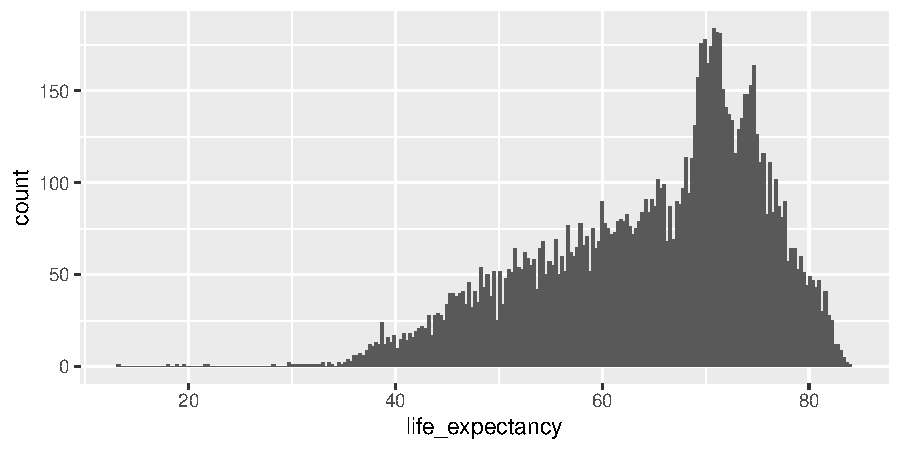
\includegraphics{skills_ps_1_files/figure-latex/unnamed-chunk-9-1.pdf}

\begin{Shaded}
\begin{Highlighting}[]
\CommentTok{# Graph 2}
\KeywordTok{ggplot}\NormalTok{(}\DataTypeTok{data =}\NormalTok{ polls_us_election_}\DecValTok{2016}\NormalTok{) }\OperatorTok{+}
\StringTok{  }\KeywordTok{geom_point}\NormalTok{(}\DataTypeTok{mapping =} \KeywordTok{aes}\NormalTok{(}\DataTypeTok{x =}\NormalTok{ startdate, }
                           \DataTypeTok{y =}\NormalTok{ samplesize, }
                           \DataTypeTok{color =} \KeywordTok{as.character}\NormalTok{(rawpoll_johnson)))}
\end{Highlighting}
\end{Shaded}

\begin{verbatim}
## Warning: Removed 1 rows containing missing values (geom_point).
\end{verbatim}

  \includegraphics{skills_ps_1_files/figure-latex/unnamed-chunk-9-2.pdf}

\begin{Shaded}
\begin{Highlighting}[]
\CommentTok{# The two graphs differ in how they assign colors to the data points of}
\CommentTok{# rawpoll_johnson. Graph 1 assigns a blue color to rawpoll_johnson that gets}
\CommentTok{# lighter in color as value increases. Graph 2 assigns a new color to each }
\CommentTok{# unique 'character' in the variable rawpoll_johnson. Graph 1 is a better}
\CommentTok{# representation of the data because it shows the raw poll scores fit in a }
\CommentTok{# chart of start date versus sample size.}
\end{Highlighting}
\end{Shaded}
\item
  What happens if you map an aesthetic to something other than a
  variable name, like
  \texttt{aes(color\ =\ samplesize\ \textgreater{}=\ 500)}

\begin{Shaded}
\begin{Highlighting}[]
\KeywordTok{ggplot}\NormalTok{(}\DataTypeTok{data =}\NormalTok{ polls_us_election_}\DecValTok{2016}\NormalTok{) }\OperatorTok{+}
\StringTok{  }\KeywordTok{geom_point}\NormalTok{(}\DataTypeTok{mapping =} \KeywordTok{aes}\NormalTok{(}\DataTypeTok{x =}\NormalTok{ startdate, }
                           \DataTypeTok{y =}\NormalTok{ rawpoll_clinton, }
                           \DataTypeTok{color =}\NormalTok{ samplesize }\OperatorTok{>=}\StringTok{ }\DecValTok{500}\NormalTok{))}
\end{Highlighting}
\end{Shaded}

  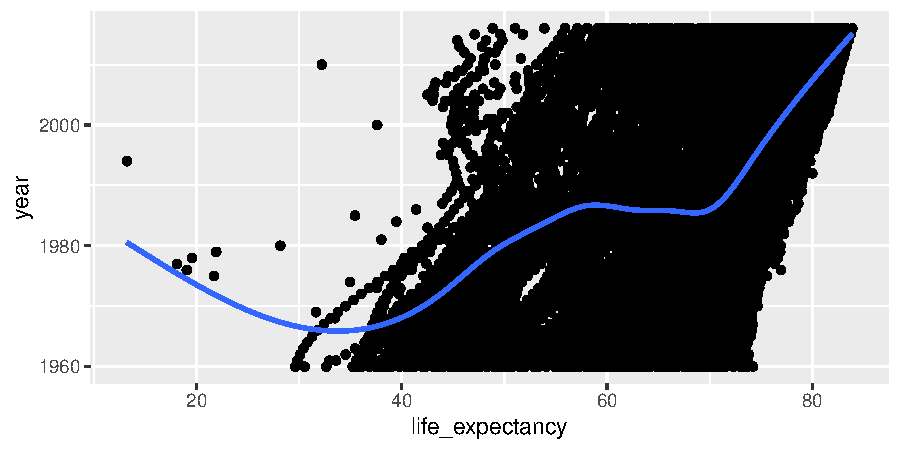
\includegraphics{skills_ps_1_files/figure-latex/unnamed-chunk-10-1.pdf}

\begin{Shaded}
\begin{Highlighting}[]
\CommentTok{# When an aesthetic is mapped to something other than a variable name, such }
\CommentTok{# as `color = samplesize >= 500`, you can differentiate the data by color }
\CommentTok{# which pollsters had sample size over a specific size. This means you can }
\CommentTok{# create a threshold and visually observe differences by color in the plot.}
\end{Highlighting}
\end{Shaded}
\item
  Common bugs: What's gone wrong with this code? Fix the code so the
  points are blue.

\begin{Shaded}
\begin{Highlighting}[]
\CommentTok{# ggplot(data = polls_us_election_2016) + }
\CommentTok{#  geom_point(mapping = aes(x = startdate, }
\CommentTok{#                           y = rawpoll_clinton, }
\CommentTok{#                           color = "blue"))}

\KeywordTok{ggplot}\NormalTok{(}\DataTypeTok{data =}\NormalTok{ polls_us_election_}\DecValTok{2016}\NormalTok{) }\OperatorTok{+}\StringTok{ }
\StringTok{  }\KeywordTok{geom_point}\NormalTok{(}\DataTypeTok{mapping =} \KeywordTok{aes}\NormalTok{(}\DataTypeTok{x =}\NormalTok{ startdate, }
                           \DataTypeTok{y =}\NormalTok{ rawpoll_clinton),}
                           \DataTypeTok{color =} \StringTok{"blue"}\NormalTok{)}
\end{Highlighting}
\end{Shaded}

  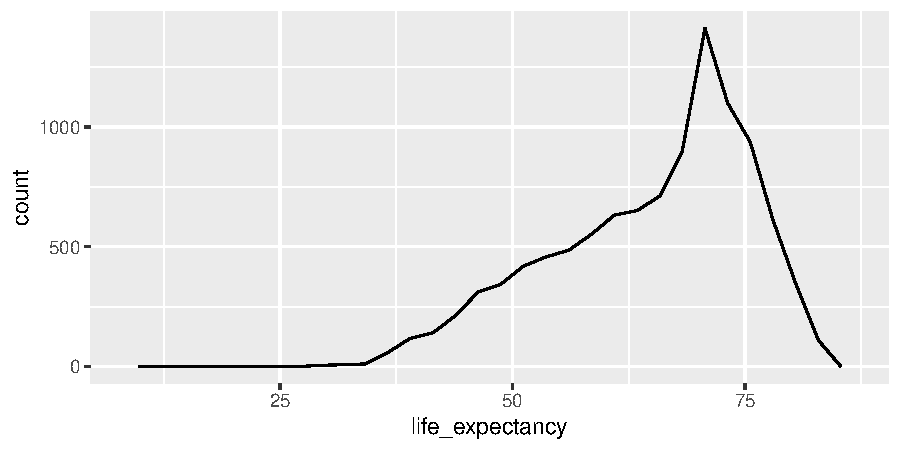
\includegraphics{skills_ps_1_files/figure-latex/unnamed-chunk-11-1.pdf}
\end{enumerate}

\hypertarget{grammar-of-graphics-facets-20-points}{%
\subsection{grammar of graphics: Facets (20
points)}\label{grammar-of-graphics-facets-20-points}}

\begin{enumerate}
\def\labelenumi{\arabic{enumi}.}
\item
  Make the following plots. How does \texttt{facet\_grid()} decide the
  layout of the grid?

\begin{Shaded}
\begin{Highlighting}[]
\KeywordTok{ggplot}\NormalTok{(}\DataTypeTok{data =}\NormalTok{ polls_us_election_}\DecValTok{2016}\NormalTok{) }\OperatorTok{+}\StringTok{ }
\StringTok{  }\KeywordTok{geom_point}\NormalTok{(}\DataTypeTok{mapping =} \KeywordTok{aes}\NormalTok{(}\DataTypeTok{x =}\NormalTok{ startdate, }
                           \DataTypeTok{y =}\NormalTok{ rawpoll_clinton)) }\OperatorTok{+}
\StringTok{  }\KeywordTok{facet_grid}\NormalTok{(}\DataTypeTok{cols =} \KeywordTok{vars}\NormalTok{(population))}
\end{Highlighting}
\end{Shaded}

  \includegraphics{skills_ps_1_files/figure-latex/unnamed-chunk-12-1.pdf}

\begin{Shaded}
\begin{Highlighting}[]
\KeywordTok{ggplot}\NormalTok{(}\DataTypeTok{data =}\NormalTok{ polls_us_election_}\DecValTok{2016}\NormalTok{) }\OperatorTok{+}\StringTok{ }
\StringTok{  }\KeywordTok{geom_point}\NormalTok{(}\DataTypeTok{mapping =} \KeywordTok{aes}\NormalTok{(}\DataTypeTok{x =}\NormalTok{ startdate, }
                           \DataTypeTok{y =}\NormalTok{ rawpoll_clinton)) }\OperatorTok{+}
\StringTok{  }\KeywordTok{facet_grid}\NormalTok{(}\DataTypeTok{rows =} \KeywordTok{vars}\NormalTok{(grade))}
\end{Highlighting}
\end{Shaded}

  \includegraphics{skills_ps_1_files/figure-latex/unnamed-chunk-12-2.pdf}

\begin{Shaded}
\begin{Highlighting}[]
\KeywordTok{ggplot}\NormalTok{(}\DataTypeTok{data =}\NormalTok{ polls_us_election_}\DecValTok{2016}\NormalTok{) }\OperatorTok{+}\StringTok{ }
\StringTok{  }\KeywordTok{geom_point}\NormalTok{(}\DataTypeTok{mapping =} \KeywordTok{aes}\NormalTok{(}\DataTypeTok{x =}\NormalTok{ startdate, }
                           \DataTypeTok{y =}\NormalTok{ rawpoll_clinton)) }\OperatorTok{+}
\StringTok{  }\KeywordTok{facet_grid}\NormalTok{(}\DataTypeTok{rows =} \KeywordTok{vars}\NormalTok{(grade), }\DataTypeTok{cols =} \KeywordTok{vars}\NormalTok{(population))}
\end{Highlighting}
\end{Shaded}

  \includegraphics{skills_ps_1_files/figure-latex/unnamed-chunk-12-3.pdf}

\begin{Shaded}
\begin{Highlighting}[]
\CommentTok{# `facet_grid()` decide the layout of the grid using vars(), which tells }
\CommentTok{# which variables to include/exclude in the plot as a column or row.}
\end{Highlighting}
\end{Shaded}
\item
  What happens if you facet a continuous variable? Provide an example
\end{enumerate}

\begin{Shaded}
\begin{Highlighting}[]
\CommentTok{# if you facet a continuous variable, it can create very many segments of }
\CommentTok{# rows/columns depending on what you assign in facet_grid(). The following code }
\CommentTok{# in comment is my example of faceting a continuous variable (not run due to }
\CommentTok{# crashing Rstudio)}

\CommentTok{#    ggplot(data = polls_us_election_2016) + }
\CommentTok{#      geom_point(mapping = aes(x = startdate, }
\CommentTok{#                               y = population)) +}
\CommentTok{#      facet_grid(rows = vars(rawpoll_trump))}
\CommentTok{#}
\CommentTok{# we adjust our code to only see a segment data to facet a continuous variable}

\NormalTok{facet_continuous_variable <-}\StringTok{ }\KeywordTok{head}\NormalTok{(polls_us_election_}\DecValTok{2016}\NormalTok{)}

    \KeywordTok{ggplot}\NormalTok{(}\DataTypeTok{data =}\NormalTok{ facet_continuous_variable) }\OperatorTok{+}\StringTok{ }
\StringTok{      }\KeywordTok{geom_point}\NormalTok{(}\DataTypeTok{mapping =} \KeywordTok{aes}\NormalTok{(}\DataTypeTok{x =}\NormalTok{ startdate, }
                               \DataTypeTok{y =}\NormalTok{ rawpoll_trump)) }\OperatorTok{+}
\StringTok{      }\KeywordTok{facet_grid}\NormalTok{(}\DataTypeTok{rows =} \KeywordTok{vars}\NormalTok{(rawpoll_trump))}
\end{Highlighting}
\end{Shaded}

\includegraphics{skills_ps_1_files/figure-latex/unnamed-chunk-13-1.pdf}
1. Reproduce the following graph

\begin{Shaded}
\begin{Highlighting}[]
\KeywordTok{ggplot}\NormalTok{(}\DataTypeTok{data =}\NormalTok{ polls_us_election_}\DecValTok{2016}\NormalTok{) }\OperatorTok{+}
\StringTok{      }\KeywordTok{geom_point}\NormalTok{(}\KeywordTok{aes}\NormalTok{(}\DataTypeTok{x =}\NormalTok{ startdate, }
                     \DataTypeTok{y =}\NormalTok{ rawpoll_trump, }
                     \DataTypeTok{color =}\NormalTok{ grade)) }\OperatorTok{+}
\StringTok{      }\KeywordTok{facet_grid}\NormalTok{(}\DataTypeTok{rows =} \KeywordTok{vars}\NormalTok{(population))}
\end{Highlighting}
\end{Shaded}

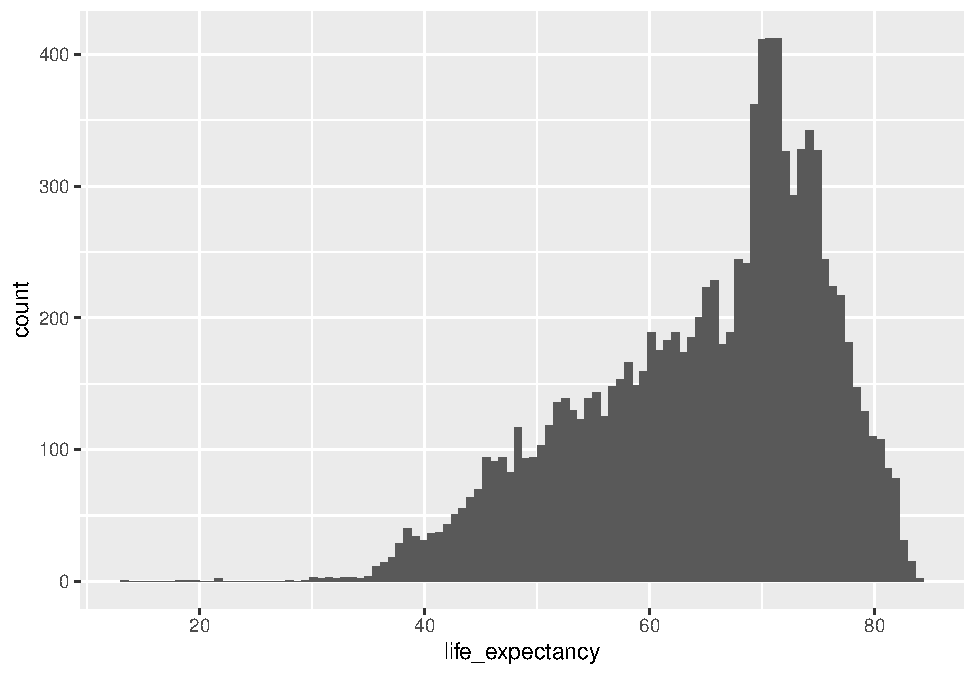
\includegraphics{skills_ps_1_files/figure-latex/unnamed-chunk-14-1.pdf}

\begin{Shaded}
\begin{Highlighting}[]
\CommentTok{# Similarly, the graph produced from the above code can also be produced for }
    \CommentTok{# Clinton and other candidates}
    
        \KeywordTok{ggplot}\NormalTok{(}\DataTypeTok{data =}\NormalTok{ polls_us_election_}\DecValTok{2016}\NormalTok{) }\OperatorTok{+}
\StringTok{      }\KeywordTok{geom_point}\NormalTok{(}\KeywordTok{aes}\NormalTok{(}\DataTypeTok{x =}\NormalTok{ startdate, }
                     \DataTypeTok{y =}\NormalTok{ rawpoll_clinton, }
                     \DataTypeTok{color =}\NormalTok{ grade)) }\OperatorTok{+}
\StringTok{      }\KeywordTok{facet_grid}\NormalTok{(}\DataTypeTok{rows =} \KeywordTok{vars}\NormalTok{(population))}
\end{Highlighting}
\end{Shaded}

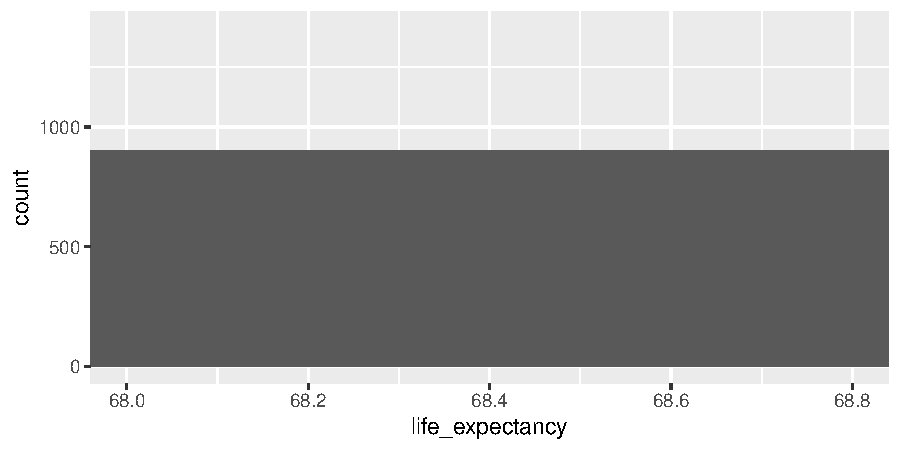
\includegraphics{skills_ps_1_files/figure-latex/unnamed-chunk-15-1.pdf}

\begin{enumerate}
\def\labelenumi{\arabic{enumi}.}
\tightlist
\item
  Rotate 45 degrees the \texttt{startdate} labels from the previous
  plot. You can use Google, include \texttt{ggplot} in your search to
  get more relevant answers. Remember to cite any code you gather from
  the internet.
\end{enumerate}

\begin{Shaded}
\begin{Highlighting}[]
\CommentTok{#our goal is to rotate x axis labels 45 degrees}
\CommentTok{#code_source: }
\CommentTok{#https://stackoverflow.com/questions/1330989/rotating-and-spacing-axis-labels-in-ggplot2}

    \KeywordTok{ggplot}\NormalTok{(}\DataTypeTok{data =}\NormalTok{ polls_us_election_}\DecValTok{2016}\NormalTok{) }\OperatorTok{+}
\StringTok{      }\KeywordTok{geom_point}\NormalTok{(}\KeywordTok{aes}\NormalTok{(}\DataTypeTok{x =}\NormalTok{ startdate, }
                     \DataTypeTok{y =}\NormalTok{ rawpoll_trump, }
                     \DataTypeTok{color =}\NormalTok{ grade)) }\OperatorTok{+}
\StringTok{      }\KeywordTok{facet_grid}\NormalTok{(}\DataTypeTok{rows =} \KeywordTok{vars}\NormalTok{(population)) }\OperatorTok{+}\StringTok{ }\KeywordTok{theme}\NormalTok{(}
        \DataTypeTok{axis.text.x =} \KeywordTok{element_text}\NormalTok{(}\DataTypeTok{angle =} \DecValTok{45}\NormalTok{, }\DataTypeTok{vjust =} \FloatTok{0.5}\NormalTok{, }\DataTypeTok{hjust=}\DecValTok{1}\NormalTok{))}
\end{Highlighting}
\end{Shaded}

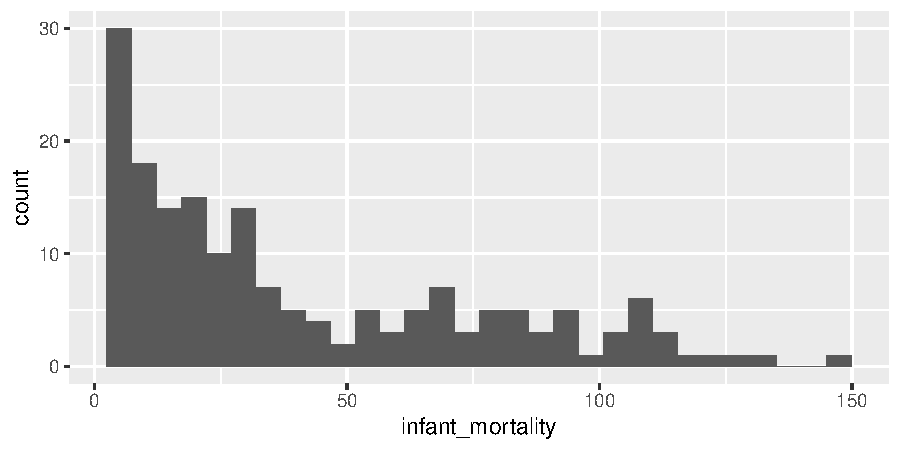
\includegraphics{skills_ps_1_files/figure-latex/unnamed-chunk-16-1.pdf}

\begin{enumerate}
\def\labelenumi{\arabic{enumi}.}
\item
  Reproduce the following graph. Why are there grades missing?

\begin{Shaded}
\begin{Highlighting}[]
\KeywordTok{ggplot}\NormalTok{(}\DataTypeTok{data =}\NormalTok{ polls_us_election_}\DecValTok{2016}\NormalTok{) }\OperatorTok{+}
\StringTok{  }\KeywordTok{geom_point}\NormalTok{(}\KeywordTok{aes}\NormalTok{(}\DataTypeTok{x =}\NormalTok{ startdate, }
             \DataTypeTok{y =}\NormalTok{ rawpoll_clinton,}
             \DataTypeTok{shape =}\NormalTok{ grade)) }\OperatorTok{+}
\StringTok{  }\KeywordTok{facet_grid}\NormalTok{(}\DataTypeTok{rows =} \KeywordTok{vars}\NormalTok{(population))}
\end{Highlighting}
\end{Shaded}

\begin{verbatim}
## Warning: The shape palette can deal with a maximum of 6 discrete values because
## more than 6 becomes difficult to discriminate; you have 10. Consider
## specifying shapes manually if you must have them.
\end{verbatim}

\begin{verbatim}
## Warning: Removed 1961 rows containing missing values (geom_point).
\end{verbatim}

  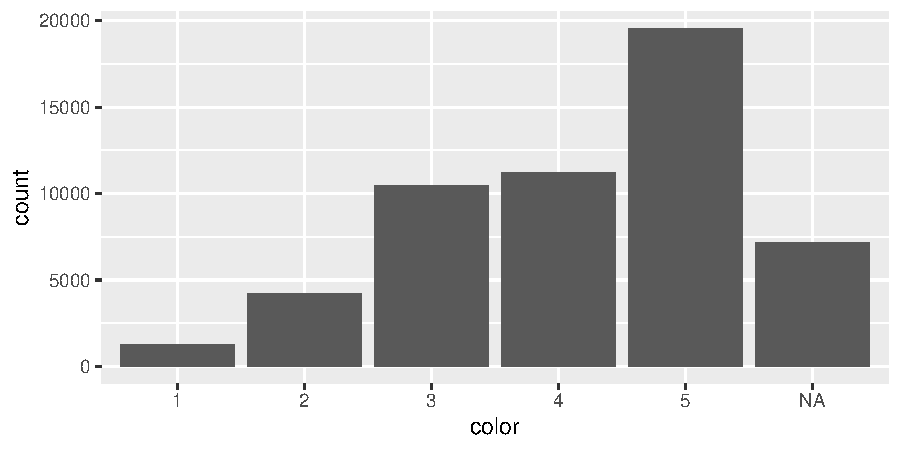
\includegraphics{skills_ps_1_files/figure-latex/unnamed-chunk-17-1.pdf}

\begin{Shaded}
\begin{Highlighting}[]
\CommentTok{# There appears to be limited number of shapes stored in R, less than the }
\CommentTok{# total number of grades.}
\end{Highlighting}
\end{Shaded}
\end{enumerate}

\hypertarget{grammar-of-graphics-geoms-10-pts}{%
\subsection{\texorpdfstring{Grammar of graphics: \texttt{geom}s (10
pts)}{Grammar of graphics: geoms (10 pts)}}\label{grammar-of-graphics-geoms-10-pts}}

\begin{enumerate}
\def\labelenumi{\arabic{enumi}.}
\tightlist
\item
  What geom would you use to draw a line chart? A boxplot? A histogram?
  An area chart?
\end{enumerate}

\begin{Shaded}
\begin{Highlighting}[]
\CommentTok{# to draw a line chart, use geom_line()}
\CommentTok{# to draw a boxplot, use geom_boxplot()}
\CommentTok{# to draw a histogram, use geom_histogram()}
\CommentTok{# to draw an area chart, use geom_area()}
\end{Highlighting}
\end{Shaded}

\begin{enumerate}
\def\labelenumi{\arabic{enumi}.}
\item
  Will these two graphs look different? Why/why not?

\begin{Shaded}
\begin{Highlighting}[]
\KeywordTok{ggplot}\NormalTok{(}\DataTypeTok{data =}\NormalTok{ polls_us_election_}\DecValTok{2016}\NormalTok{, }
       \DataTypeTok{mapping =} \KeywordTok{aes}\NormalTok{(}\DataTypeTok{x =}\NormalTok{ startdate, }
                     \DataTypeTok{y =}\NormalTok{ rawpoll_trump)) }\OperatorTok{+}
\StringTok{  }\KeywordTok{geom_point}\NormalTok{() }\OperatorTok{+}
\StringTok{  }\KeywordTok{geom_smooth}\NormalTok{(}\DataTypeTok{se=}\OtherTok{FALSE}\NormalTok{)}
\end{Highlighting}
\end{Shaded}

\begin{verbatim}
## `geom_smooth()` using method = 'gam' and formula 'y ~ s(x, bs = "cs")'
\end{verbatim}

  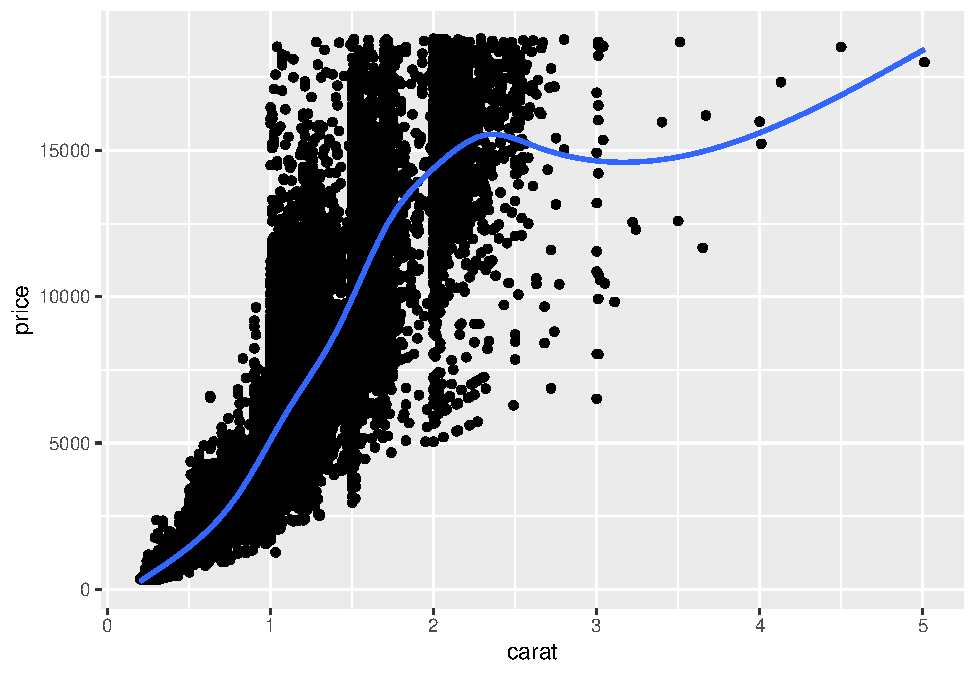
\includegraphics{skills_ps_1_files/figure-latex/unnamed-chunk-19-1.pdf}

\begin{Shaded}
\begin{Highlighting}[]
\KeywordTok{ggplot}\NormalTok{() }\OperatorTok{+}
\StringTok{  }\KeywordTok{geom_point}\NormalTok{(}\DataTypeTok{data =}\NormalTok{ polls_us_election_}\DecValTok{2016}\NormalTok{, }
             \DataTypeTok{mapping =} \KeywordTok{aes}\NormalTok{(}\DataTypeTok{x =}\NormalTok{ startdate, }
                           \DataTypeTok{y =}\NormalTok{ rawpoll_trump)) }\OperatorTok{+}
\StringTok{  }\KeywordTok{geom_smooth}\NormalTok{(}\DataTypeTok{data =}\NormalTok{ polls_us_election_}\DecValTok{2016}\NormalTok{, }
              \DataTypeTok{mapping =} \KeywordTok{aes}\NormalTok{(}\DataTypeTok{x =}\NormalTok{ startdate, }
                            \DataTypeTok{y =}\NormalTok{ rawpoll_trump), }\DataTypeTok{se=}\OtherTok{FALSE}\NormalTok{)}
\end{Highlighting}
\end{Shaded}

\begin{verbatim}
## `geom_smooth()` using method = 'gam' and formula 'y ~ s(x, bs = "cs")'
\end{verbatim}

  \includegraphics{skills_ps_1_files/figure-latex/unnamed-chunk-19-2.pdf}

\begin{Shaded}
\begin{Highlighting}[]
\CommentTok{# these two graphs are identical even if their codes are slightly different.}
\CommentTok{# Duplicative code can be removed to achieve the same plot. In this case,}
\CommentTok{# data = polls_us_election_2016, }
\CommentTok{#              mapping = aes(x = startdate, }
\CommentTok{#                            y = rawpoll_trump}
\CommentTok{# is duplicative and only has to be coded into one of the following to work:}
\CommentTok{# ggplot(), geom_point(), and geom_smooth().}
\end{Highlighting}
\end{Shaded}
\end{enumerate}

\begin{Shaded}
\begin{Highlighting}[]
\CommentTok{# Below is the previous code with the data syntax entered into all three }
\CommentTok{# functions, producing the identical plot still.}

 \KeywordTok{ggplot}\NormalTok{(}\DataTypeTok{data =}\NormalTok{ polls_us_election_}\DecValTok{2016}\NormalTok{, }
                 \DataTypeTok{mapping =} \KeywordTok{aes}\NormalTok{(}\DataTypeTok{x =}\NormalTok{ startdate, }
                               \DataTypeTok{y =}\NormalTok{ rawpoll_trump)) }\OperatorTok{+}
\StringTok{      }\KeywordTok{geom_point}\NormalTok{(}\DataTypeTok{data =}\NormalTok{ polls_us_election_}\DecValTok{2016}\NormalTok{, }
                 \DataTypeTok{mapping =} \KeywordTok{aes}\NormalTok{(}\DataTypeTok{x =}\NormalTok{ startdate, }
                               \DataTypeTok{y =}\NormalTok{ rawpoll_trump)) }\OperatorTok{+}
\StringTok{      }\KeywordTok{geom_smooth}\NormalTok{(}\DataTypeTok{data =}\NormalTok{ polls_us_election_}\DecValTok{2016}\NormalTok{, }
                  \DataTypeTok{mapping =} \KeywordTok{aes}\NormalTok{(}\DataTypeTok{x =}\NormalTok{ startdate, }
                                \DataTypeTok{y =}\NormalTok{ rawpoll_trump), }\DataTypeTok{se=}\OtherTok{FALSE}\NormalTok{)}
\end{Highlighting}
\end{Shaded}

\begin{verbatim}
## `geom_smooth()` using method = 'gam' and formula 'y ~ s(x, bs = "cs")'
\end{verbatim}

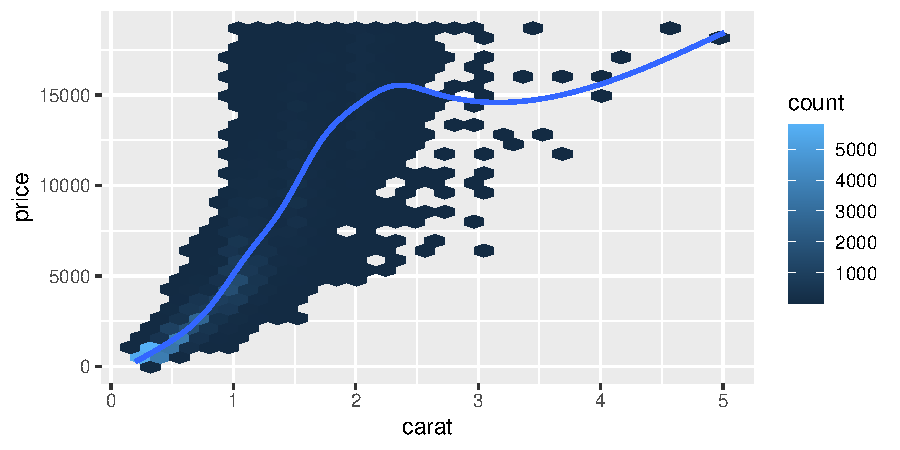
\includegraphics{skills_ps_1_files/figure-latex/unnamed-chunk-20-1.pdf}
1. You are trying to figure out if there is a relationship between Trump
poll numbers and the quality of the polls. Write code to make this
graph.

\begin{Shaded}
\begin{Highlighting}[]
    \KeywordTok{ggplot}\NormalTok{(}\DataTypeTok{data =}\NormalTok{ polls_us_election_}\DecValTok{2016}\NormalTok{, }
           \DataTypeTok{mapping =} \KeywordTok{aes}\NormalTok{(}\DataTypeTok{x =}\NormalTok{ startdate, }
                         \DataTypeTok{y =}\NormalTok{ rawpoll_trump)) }\OperatorTok{+}
\StringTok{        }\KeywordTok{geom_point}\NormalTok{(}\KeywordTok{aes}\NormalTok{(}\DataTypeTok{color =}\NormalTok{ grade)) }\OperatorTok{+}
\StringTok{        }\KeywordTok{geom_smooth}\NormalTok{(}\DataTypeTok{se =} \OtherTok{FALSE}\NormalTok{)}
\end{Highlighting}
\end{Shaded}

\begin{verbatim}
## `geom_smooth()` using method = 'gam' and formula 'y ~ s(x, bs = "cs")'
\end{verbatim}

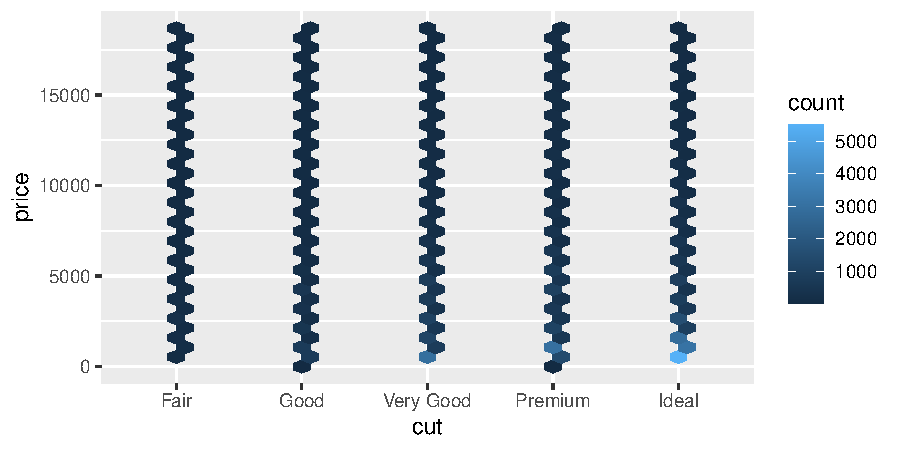
\includegraphics{skills_ps_1_files/figure-latex/unnamed-chunk-21-1.pdf}

\begin{enumerate}
\def\labelenumi{\arabic{enumi}.}
\tightlist
\item
  Make some changes to this graph:

  \begin{itemize}
  \tightlist
  \item
    make line red
  \item
    make the x- and y-axes labels more informative using
    \texttt{+\ labs()}
  \item
    use an informative title
  \item
    remove the legend (Google might be helpful to learn how) Are all
    four changes improvements? Which change made the plot worse and why?
  \end{itemize}
\end{enumerate}

\begin{Shaded}
\begin{Highlighting}[]
    \KeywordTok{ggplot}\NormalTok{(}\DataTypeTok{data =}\NormalTok{ polls_us_election_}\DecValTok{2016}\NormalTok{, }
           \DataTypeTok{mapping =} \KeywordTok{aes}\NormalTok{(}\DataTypeTok{x =}\NormalTok{ startdate, }
                         \DataTypeTok{y =}\NormalTok{ rawpoll_trump)) }\OperatorTok{+}
\StringTok{        }\KeywordTok{geom_point}\NormalTok{(}\KeywordTok{aes}\NormalTok{(}\DataTypeTok{color =}\NormalTok{ grade), }\DataTypeTok{show.legend =} \OtherTok{FALSE}\NormalTok{) }\OperatorTok{+}
\StringTok{        }\KeywordTok{geom_smooth}\NormalTok{(}\DataTypeTok{se =} \OtherTok{FALSE}\NormalTok{, }\DataTypeTok{color =} \StringTok{"Red"}\NormalTok{) }\OperatorTok{+}\StringTok{ }\KeywordTok{labs}\NormalTok{(}\DataTypeTok{title=}\StringTok{"Plot of Pollster }
\StringTok{                                                      Scores by Start Date"}\NormalTok{,}
        \DataTypeTok{x =}\StringTok{"Start Date"}\NormalTok{, }\DataTypeTok{y =} \StringTok{"Raw Poll Score"}\NormalTok{)}
\end{Highlighting}
\end{Shaded}

\begin{verbatim}
## `geom_smooth()` using method = 'gam' and formula 'y ~ s(x, bs = "cs")'
\end{verbatim}

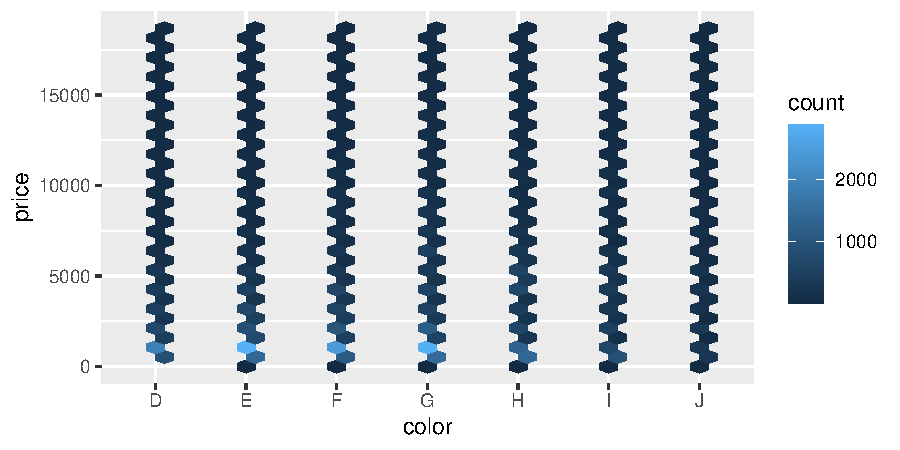
\includegraphics{skills_ps_1_files/figure-latex/unnamed-chunk-22-1.pdf}

\begin{Shaded}
\begin{Highlighting}[]
\CommentTok{# All changes except removal of the legend I think are improvements to make the }
\CommentTok{# data and chart clearer.}
\CommentTok{# Removing the legend was not an improvement because by removing it we lose the }
\CommentTok{# association of each color to each grade.}
\end{Highlighting}
\end{Shaded}

\hypertarget{grammar-of-graphics-statistical-transformations-10-pts}{%
\subsubsection{grammar of graphics: Statistical transformations (10
pts)}\label{grammar-of-graphics-statistical-transformations-10-pts}}

\begin{enumerate}
\def\labelenumi{\arabic{enumi}.}
\tightlist
\item
  What does \texttt{geom\_col()} do? How is it different from
  \texttt{geom\_bar()}?
\end{enumerate}

\begin{Shaded}
\begin{Highlighting}[]
\CommentTok{#link: https://ggplot2.tidyverse.org/reference/geom_bar.html}
\NormalTok{?}\KeywordTok{geom_bar}\NormalTok{()}
\NormalTok{?}\KeywordTok{geom_col}\NormalTok{()}

\CommentTok{# geom_col and geom_bar are two types of bar charts in R. In my own words,}
\CommentTok{# with geom_col you can plot values of any x variable against any y variable.}
\CommentTok{# With geom_bar, you can easily plot the total count of each unique observation}
\CommentTok{# for a variable (or the number of cases at each x position). This is made}
\CommentTok{# possible by what each stat function each geom uses by default. By default,}
\CommentTok{# geom_bar uses stat_count and geom_col uses stat_identity.}

\NormalTok{example <-}\StringTok{ }\KeywordTok{tail}\NormalTok{(polls_us_election_}\DecValTok{2016}\NormalTok{)}
  
\KeywordTok{ggplot}\NormalTok{(}\DataTypeTok{data=}\NormalTok{example, }\KeywordTok{aes}\NormalTok{(}\DataTypeTok{x=}\NormalTok{pollster, }\DataTypeTok{y =}\NormalTok{ samplesize)) }\OperatorTok{+}\StringTok{ }\KeywordTok{geom_col}\NormalTok{()}\OperatorTok{+}\StringTok{ }
\StringTok{  }\KeywordTok{theme}\NormalTok{(}\DataTypeTok{axis.text.x =} \KeywordTok{element_text}\NormalTok{(}\DataTypeTok{angle =} \DecValTok{45}\NormalTok{, }\DataTypeTok{vjust =} \FloatTok{0.5}\NormalTok{, }\DataTypeTok{hjust=}\FloatTok{0.4}\NormalTok{))}
\end{Highlighting}
\end{Shaded}

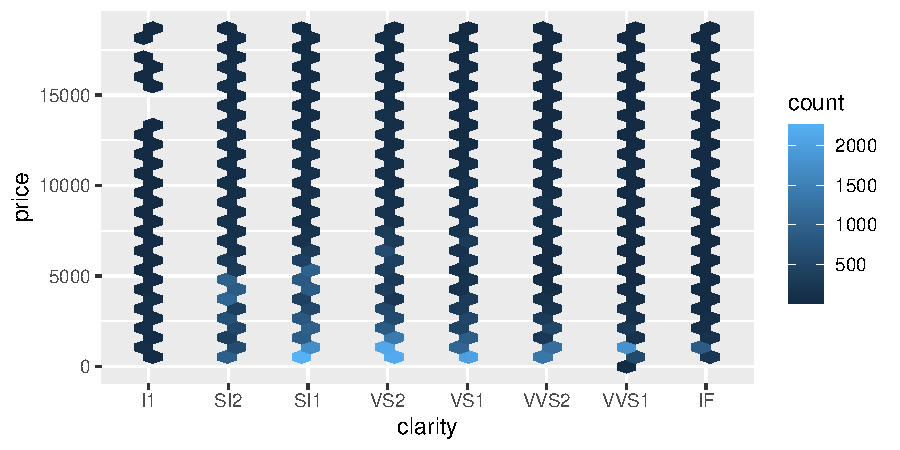
\includegraphics{skills_ps_1_files/figure-latex/unnamed-chunk-23-1.pdf}

\begin{Shaded}
\begin{Highlighting}[]
\KeywordTok{ggplot}\NormalTok{(}\DataTypeTok{data=}\NormalTok{polls_us_election_}\DecValTok{2016}\NormalTok{, }\KeywordTok{aes}\NormalTok{(}\DataTypeTok{x=}\NormalTok{grade)) }\OperatorTok{+}\StringTok{ }\KeywordTok{geom_bar}\NormalTok{()}
\end{Highlighting}
\end{Shaded}

\includegraphics{skills_ps_1_files/figure-latex/unnamed-chunk-23-2.pdf}

\begin{enumerate}
\def\labelenumi{\arabic{enumi}.}
\tightlist
\item
  Plot
  \texttt{ggplot(data=polls\_us\_election\_2016,\ aes(x=grade))\ +\ geom\_bar()}.
  Replace the \texttt{geom} with a \texttt{stat} to make the same graph.
\end{enumerate}

\begin{Shaded}
\begin{Highlighting}[]
\KeywordTok{ggplot}\NormalTok{(}\DataTypeTok{data=}\NormalTok{polls_us_election_}\DecValTok{2016}\NormalTok{, }\KeywordTok{aes}\NormalTok{(}\DataTypeTok{x=}\NormalTok{grade)) }\OperatorTok{+}\StringTok{ }\KeywordTok{geom_bar}\NormalTok{()}
\end{Highlighting}
\end{Shaded}

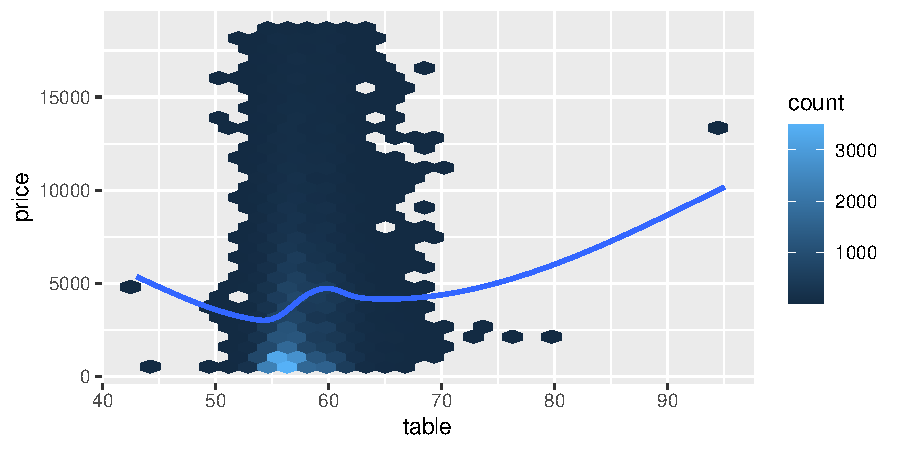
\includegraphics{skills_ps_1_files/figure-latex/unnamed-chunk-24-1.pdf}

\begin{Shaded}
\begin{Highlighting}[]
\KeywordTok{ggplot}\NormalTok{(}\DataTypeTok{data=}\NormalTok{polls_us_election_}\DecValTok{2016}\NormalTok{, }\KeywordTok{aes}\NormalTok{(}\DataTypeTok{x=}\NormalTok{grade)) }\OperatorTok{+}\StringTok{ }\KeywordTok{stat_count}\NormalTok{()}
\end{Highlighting}
\end{Shaded}

\includegraphics{skills_ps_1_files/figure-latex/unnamed-chunk-24-2.pdf}

\begin{enumerate}
\def\labelenumi{\arabic{enumi}.}
\tightlist
\item
  Which 4 variables does \texttt{stat\_smooth()} compute? How are these
  variables displayed on a graph made with \texttt{geom\_smooth()}? What
  parameters (i.e.~inputs to the function) control its behavior?
\end{enumerate}

\begin{Shaded}
\begin{Highlighting}[]
\NormalTok{?}\KeywordTok{stat_smooth}\NormalTok{()}
\NormalTok{?}\KeywordTok{geom_smooth}\NormalTok{()}

\CommentTok{# Computed variables are the same for both functions.}
\CommentTok{## y = predicted value}

\CommentTok{## ymin = lower pointwise confidence interval around the mean}

\CommentTok{## ymax = upper pointwise confidence interval around the mean}

\CommentTok{## se = standard error}

\CommentTok{# If we want to display our results with a non-standard geom, we use}
\CommentTok{# stat_smooth().}

\CommentTok{# Their parameters (inputs) that control its behavior are shown in full below:}

\KeywordTok{geom_smooth}\NormalTok{(}
  \DataTypeTok{mapping =} \OtherTok{NULL}\NormalTok{,}
  \DataTypeTok{data =} \OtherTok{NULL}\NormalTok{,}
  \DataTypeTok{stat =} \StringTok{"smooth"}\NormalTok{,}
  \DataTypeTok{position =} \StringTok{"identity"}\NormalTok{,}
\NormalTok{  ...,}
  \DataTypeTok{method =} \OtherTok{NULL}\NormalTok{,}
  \DataTypeTok{formula =} \OtherTok{NULL}\NormalTok{,}
  \DataTypeTok{se =} \OtherTok{TRUE}\NormalTok{,}
  \DataTypeTok{na.rm =} \OtherTok{FALSE}\NormalTok{,}
  \DataTypeTok{orientation =} \OtherTok{NA}\NormalTok{,}
  \DataTypeTok{show.legend =} \OtherTok{NA}\NormalTok{,}
  \DataTypeTok{inherit.aes =} \OtherTok{TRUE}
\NormalTok{)}

\KeywordTok{stat_smooth}\NormalTok{(}
  \DataTypeTok{mapping =} \OtherTok{NULL}\NormalTok{,}
  \DataTypeTok{data =} \OtherTok{NULL}\NormalTok{,}
  \DataTypeTok{geom =} \StringTok{"smooth"}\NormalTok{,}
  \DataTypeTok{position =} \StringTok{"identity"}\NormalTok{,}
\NormalTok{  ...,}
  \DataTypeTok{method =} \OtherTok{NULL}\NormalTok{,}
  \DataTypeTok{formula =} \OtherTok{NULL}\NormalTok{,}
  \DataTypeTok{se =} \OtherTok{TRUE}\NormalTok{,}
  \DataTypeTok{n =} \DecValTok{80}\NormalTok{,}
  \DataTypeTok{span =} \FloatTok{0.75}\NormalTok{,}
  \DataTypeTok{fullrange =} \OtherTok{FALSE}\NormalTok{,}
  \DataTypeTok{level =} \FloatTok{0.95}\NormalTok{,}
  \DataTypeTok{method.args =} \KeywordTok{list}\NormalTok{(),}
  \DataTypeTok{na.rm =} \OtherTok{FALSE}\NormalTok{,}
  \DataTypeTok{orientation =} \OtherTok{NA}\NormalTok{,}
  \DataTypeTok{show.legend =} \OtherTok{NA}\NormalTok{,}
  \DataTypeTok{inherit.aes =} \OtherTok{TRUE}
\NormalTok{)}
\end{Highlighting}
\end{Shaded}

\begin{enumerate}
\def\labelenumi{\arabic{enumi}.}
\item
  What is wrong with the following graph? Do we need to add
  \texttt{group\ =\ 1} to it? What denominator is ggplot using to
  determine proportions?

\begin{Shaded}
\begin{Highlighting}[]
\KeywordTok{ggplot}\NormalTok{(}\DataTypeTok{data =}\NormalTok{ polls_us_election_}\DecValTok{2016}\NormalTok{) }\OperatorTok{+}\StringTok{ }
\StringTok{  }\KeywordTok{geom_bar}\NormalTok{(}\DataTypeTok{mapping =} \KeywordTok{aes}\NormalTok{(}\DataTypeTok{x =}\NormalTok{ grade, }\DataTypeTok{y =}\NormalTok{ ..prop..))}
\end{Highlighting}
\end{Shaded}

  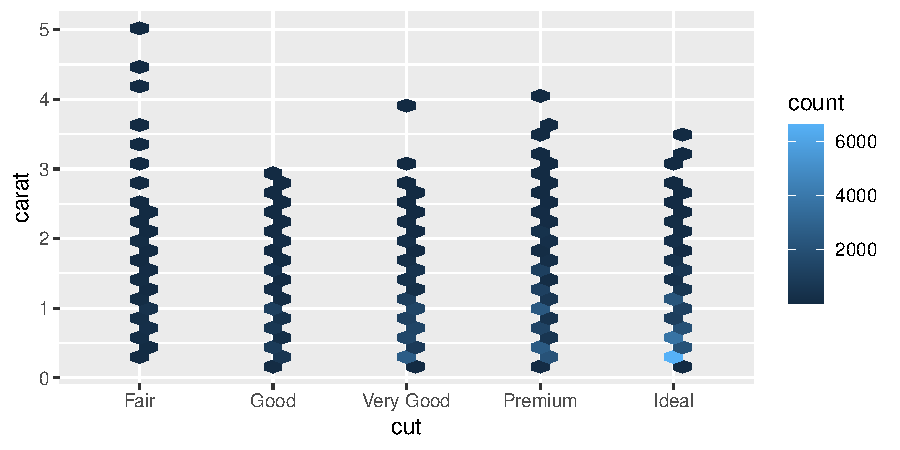
\includegraphics{skills_ps_1_files/figure-latex/unnamed-chunk-26-1.pdf}

\begin{Shaded}
\begin{Highlighting}[]
\CommentTok{# the graph before adding `group = 1` does not take into account each grades}
\CommentTok{# proportion in terms of the total dataset. It simply tells us proportion}
\CommentTok{# of each grade in terms of its own subtotal. We need to add `group = 1`, to}
\CommentTok{# observe proportion of each grade in relation to the total count of grades.}

\KeywordTok{ggplot}\NormalTok{(}\DataTypeTok{data =}\NormalTok{ polls_us_election_}\DecValTok{2016}\NormalTok{) }\OperatorTok{+}\StringTok{ }
\StringTok{  }\KeywordTok{geom_bar}\NormalTok{(}\DataTypeTok{mapping =} \KeywordTok{aes}\NormalTok{(}\DataTypeTok{x =}\NormalTok{ grade, }\DataTypeTok{y =}\NormalTok{ ..prop.., }\DataTypeTok{group =} \DecValTok{1}\NormalTok{))}
\end{Highlighting}
\end{Shaded}

  \includegraphics{skills_ps_1_files/figure-latex/unnamed-chunk-26-2.pdf}
  \#\# grammar of graphics: Positional adjustments (5 pts)
\item
  What is the problem with this plot? How could you improve it? (You
  already made this plot in this Pset)

\begin{Shaded}
\begin{Highlighting}[]
\KeywordTok{ggplot}\NormalTok{(}\DataTypeTok{data =}\NormalTok{ polls_us_election_}\DecValTok{2016}\NormalTok{, }
       \DataTypeTok{mapping =} \KeywordTok{aes}\NormalTok{(}\DataTypeTok{x =}\NormalTok{ population, }\DataTypeTok{y =}\NormalTok{ grade)) }\OperatorTok{+}\StringTok{ }
\StringTok{  }\KeywordTok{geom_point}\NormalTok{()}
\end{Highlighting}
\end{Shaded}

  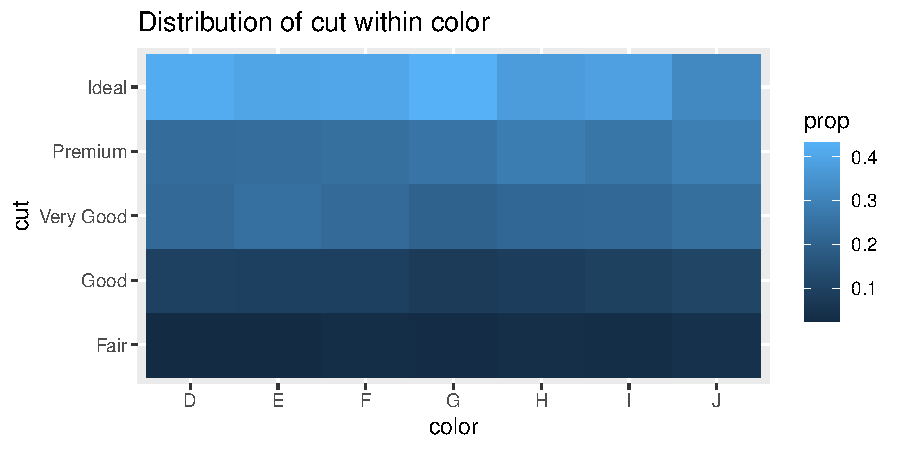
\includegraphics{skills_ps_1_files/figure-latex/unnamed-chunk-27-1.pdf}

\begin{Shaded}
\begin{Highlighting}[]
\CommentTok{# The problem with the plot from above code is that geom_point cannot show}
\CommentTok{# overlapping points, or it cannot map the number of observations at each }
\CommentTok{# point location. To improve it, we can replace geom_point for geom_count.}

    \KeywordTok{ggplot}\NormalTok{(}\DataTypeTok{data =}\NormalTok{ polls_us_election_}\DecValTok{2016}\NormalTok{, }
       \DataTypeTok{mapping =} \KeywordTok{aes}\NormalTok{(}\DataTypeTok{x =}\NormalTok{ population, }\DataTypeTok{y =}\NormalTok{ grade)) }\OperatorTok{+}\StringTok{ }
\StringTok{  }\KeywordTok{geom_count}\NormalTok{()}
\end{Highlighting}
\end{Shaded}

  \includegraphics{skills_ps_1_files/figure-latex/unnamed-chunk-27-2.pdf}
\item
  Compare and contrast \texttt{geom\_jitter()} with
  \texttt{geom\_count()}. Use vocabulary from the ``grammar of
  graphics'' to support your argument.
\end{enumerate}

\begin{Shaded}
\begin{Highlighting}[]
        \KeywordTok{ggplot}\NormalTok{(}\DataTypeTok{data =}\NormalTok{ polls_us_election_}\DecValTok{2016}\NormalTok{, }
           \DataTypeTok{mapping =} \KeywordTok{aes}\NormalTok{(}\DataTypeTok{x =}\NormalTok{ population, }\DataTypeTok{y =}\NormalTok{ grade)) }\OperatorTok{+}\StringTok{ }
\StringTok{      }\KeywordTok{geom_jitter}\NormalTok{()}
\end{Highlighting}
\end{Shaded}

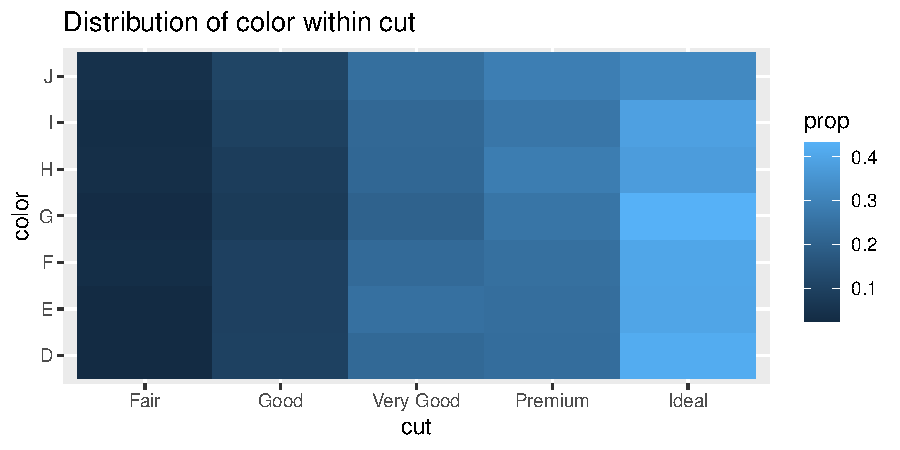
\includegraphics{skills_ps_1_files/figure-latex/unnamed-chunk-28-1.pdf}

\begin{Shaded}
\begin{Highlighting}[]
\CommentTok{# We can best compare and contrast `geom_jitter()` with `geom_count()` by first}
\CommentTok{# writing a little bit of code to produce plots for both. Overlapping is a }
\CommentTok{# challenge for our data, because there is a large number of individual grades}
\CommentTok{# and a small number of unique population values. The first plot we observe}
\CommentTok{# geom_count mapping the number of observations at each point location. This is}
\CommentTok{# helpful but it is difficult to visualize individual data points at each}
\CommentTok{# population value. We can see this better in the geom_jitter plot below, where}
\CommentTok{# a small amount of random variation is added to the location of each point.}
\end{Highlighting}
\end{Shaded}

\begin{enumerate}
\def\labelenumi{\arabic{enumi}.}
\item
  What's the default position adjustment for \texttt{geom\_bar()}? What
  did we add to the code to change the default behavior of geom\_bar?
  Here we are using the diamonds data set again

\begin{Shaded}
\begin{Highlighting}[]
\CommentTok{# reference link: https://ggplot2.tidyverse.org/reference/geom_bar.html}

\CommentTok{# the default position adjustment for `geom_bar()` is stacking. The bars are}
\CommentTok{# automatically stacked (vertically). Each color represents a unique }
\CommentTok{# observation of a variable.}
\CommentTok{# When you want to view overlapping data as side-by-side bars, you add in}
\CommentTok{# position= "dodge"}
\CommentTok{# When you want to view overlapping data as stacked bars with equal height,}
\CommentTok{# use position= "fill"}

\KeywordTok{ggplot}\NormalTok{(}\DataTypeTok{data =}\NormalTok{ diamonds) }\OperatorTok{+}\StringTok{ }
\StringTok{  }\KeywordTok{geom_bar}\NormalTok{(}\DataTypeTok{mapping =} \KeywordTok{aes}\NormalTok{(}\DataTypeTok{x =}\NormalTok{ cut, }\DataTypeTok{fill =}\NormalTok{ color, }\DataTypeTok{y =}\NormalTok{ ..prop.., }\DataTypeTok{group=}\NormalTok{ color))}
\end{Highlighting}
\end{Shaded}

  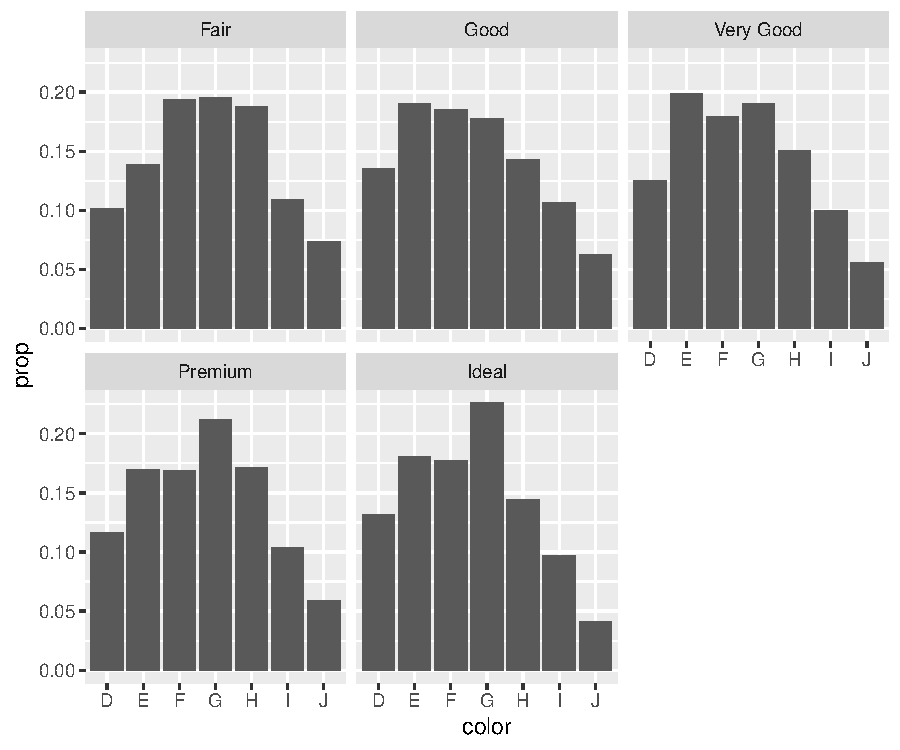
\includegraphics{skills_ps_1_files/figure-latex/unnamed-chunk-29-1.pdf}

\begin{Shaded}
\begin{Highlighting}[]
\KeywordTok{ggplot}\NormalTok{(}\DataTypeTok{data =}\NormalTok{ diamonds) }\OperatorTok{+}\StringTok{ }
\StringTok{  }\KeywordTok{geom_bar}\NormalTok{(}\DataTypeTok{mapping =} \KeywordTok{aes}\NormalTok{(}\DataTypeTok{x =}\NormalTok{ cut, }\DataTypeTok{fill =}\NormalTok{ color, }\DataTypeTok{y =}\NormalTok{ ..prop.., }\DataTypeTok{group=}\NormalTok{ color), }
           \DataTypeTok{position=}\StringTok{"dodge"}\NormalTok{)}
\end{Highlighting}
\end{Shaded}

  \includegraphics{skills_ps_1_files/figure-latex/unnamed-chunk-29-2.pdf}

\begin{Shaded}
\begin{Highlighting}[]
    \KeywordTok{ggplot}\NormalTok{(}\DataTypeTok{data =}\NormalTok{ diamonds) }\OperatorTok{+}\StringTok{ }
\StringTok{  }\KeywordTok{geom_bar}\NormalTok{(}\DataTypeTok{mapping =} \KeywordTok{aes}\NormalTok{(}\DataTypeTok{x =}\NormalTok{ cut, }\DataTypeTok{fill =}\NormalTok{ color, }\DataTypeTok{y =}\NormalTok{ ..prop.., }\DataTypeTok{group=}\NormalTok{ color), }
           \DataTypeTok{position=}\StringTok{"fill"}\NormalTok{)}
\end{Highlighting}
\end{Shaded}

  \includegraphics{skills_ps_1_files/figure-latex/unnamed-chunk-29-3.pdf}
\end{enumerate}

\hypertarget{grammar-of-graphics-coordinate-systems-5-pts}{%
\subsection{grammar of graphics: Coordinate systems (5
pts)}\label{grammar-of-graphics-coordinate-systems-5-pts}}

\begin{enumerate}
\def\labelenumi{\arabic{enumi}.}
\tightlist
\item
  What happens when you use \texttt{coord\_flip()}?
\end{enumerate}

\begin{Shaded}
\begin{Highlighting}[]
\NormalTok{?coord_flip}

\CommentTok{# coord_flip switches the cartesian coordinates of a plot, so x axis and y axis}
\CommentTok{# switch places. This is primarily useful for converting geoms and}
\CommentTok{# statistics which display y conditional on x, to x conditional on y. It also}
\CommentTok{# can be very useful for creating boxplots and other geoms in the horizontal}
\CommentTok{# instead of vertical position.}
\end{Highlighting}
\end{Shaded}

\begin{enumerate}
\def\labelenumi{\arabic{enumi}.}
\item
  What is this plot telling us? What does \texttt{geom\_abline()} do?
  Why is \texttt{coord\_fixed()} important?

\begin{Shaded}
\begin{Highlighting}[]
\KeywordTok{ggplot}\NormalTok{(}\DataTypeTok{data =}\NormalTok{ polls_us_election_}\DecValTok{2016}\NormalTok{, }
       \DataTypeTok{mapping =} \KeywordTok{aes}\NormalTok{(}\DataTypeTok{x =}\NormalTok{ rawpoll_clinton, }
                     \DataTypeTok{y =}\NormalTok{ rawpoll_trump)) }\OperatorTok{+}
\StringTok{  }\KeywordTok{geom_point}\NormalTok{() }\OperatorTok{+}\StringTok{ }
\StringTok{  }\KeywordTok{geom_abline}\NormalTok{() }\OperatorTok{+}
\StringTok{  }\KeywordTok{coord_fixed}\NormalTok{()}
\end{Highlighting}
\end{Shaded}

  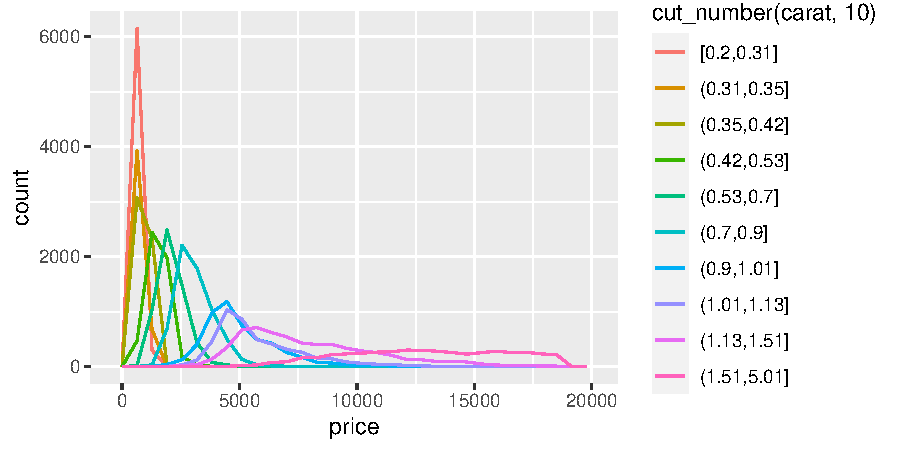
\includegraphics[width=0.5\linewidth]{skills_ps_1_files/figure-latex/unnamed-chunk-31-1}

\begin{Shaded}
\begin{Highlighting}[]
\NormalTok{?}\KeywordTok{geom_abline}\NormalTok{()}
\NormalTok{?}\KeywordTok{coord_fixed}\NormalTok{()}

\CommentTok{# This plot is telling us the raw poll scores for both Clinton and Trump for}
\CommentTok{# each pollster.}

\CommentTok{# What `geom_abline()` does is adds a reference line to the plot. Here we}
\CommentTok{# are not adding parameters to this reference line, so it starts off in its}
\CommentTok{# default slope and intercept positions, which are 1 and 0 respectively. }

\CommentTok{# The `coord_fixed()` function is important because it provides us with the}
\CommentTok{# ability to specify a ratio for the units on the x and y axes. This allows}
\CommentTok{# to stretch or widen the plot so that the resulting plot is clearer }
\CommentTok{# visually or magnified without losing integrity or accuracy in the units.}
\end{Highlighting}
\end{Shaded}
\end{enumerate}

\end{document}
